\documentclass[a4paper,14pt]{extarticle}

\usepackage{ucs}                                                                                                                   
\usepackage[utf8x]{inputenc}                                                                                                       
\usepackage[english,russian]{babel}
\usepackage[T2A]{fontenc}
\usepackage{extsizes}
\usepackage{tempora}
\usepackage[left=30mm, top=20mm, right=15mm, bottom=20mm, headheight=5pt]{geometry}
\usepackage{fancyhdr}
\usepackage{titling}
\usepackage{titlesec}
\usepackage{textcase}
\usepackage{indentfirst}
\usepackage{graphicx}
\usepackage{float}
\usepackage{caption}

\graphicspath{ {./images/} }

\newcommand{\mylabnumber}{1}
\newcommand{\mylabtitle}{Создание титульника в латеке}
\newcommand{\mysubject}{Какай-та дисциплина}
\newcommand{\mylecturer}{Захаров В.В.}

\renewcommand{\baselinestretch}{1.25} % Sets basic line stretch
\renewcommand{\headrulewidth}{0pt} % Remove horizontal line below header in fancyhdr

\addto\captionsrussian{
    \renewcommand{\figurename}{Рисунок} % Set a default picture caption
    \renewcommand{\tablename}{Таблица} % Set a default table caption
}

\captionsetup[table]{singlelinecheck=false} % To make a table caption appear left-aligned

\pagestyle{fancy}
\lhead{} \rhead{} \cfoot{} % Setting empty headers
\chead{\thepage} % Sets central header page numbering

\setlength{\parindent}{1.25cm}
\setlength{\parskip}{8pt}

\titleformat{\section}[hang]{\large \centering \bfseries}{\thesection}{0.5em}{\MakeTextUppercase} % Format section style

\titleformat{\subsection}[hang]{\bfseries}{\thesubsection}{0.5em}{} % Format subsection style
\titlespacing{\subsection}{\parindent}{1em}{1em} % Format subsection indentations

\titleformat{\subsubsection}[hang]{\normalfont}{\thesubsubsection}{0.5em}{} % Format subsubsection style
\titlespacing{\subsubsection}{\parindent}{1em}{1em} % Format subsubsection indentations

\begin{document}

    \begin{titlepage}
        
        \thispagestyle{empty}
        
        \begin{center}
            
            Министерство науки и высшего образования Российской Федерации \\
            Севастопольский государственный университет \\
            Кафедра ИС
            
            \vfill
            \large{
                Отчет \\
                по лабораторной работе №\mylabnumber \\
                "\mylabtitle" \\
                по дисциплине \\
                \MakeTextUppercase{\mysubject}
            }

        \end{center}

        \vspace{1cm}

        \noindent\hspace{7.5cm} Выполнил студент группы ИС/б-22о \\
        \null\hspace{7.5cm} Горбенко К. Н. \\
        \null\hspace{7.5cm} Проверил: \\
        \null\hspace{7.5cm} Захаров В. В.

        \vfill

        \begin{center}
            Севастополь \\
            2019
        \end{center}

    \end{titlepage}

    \section{First section}

    Hello, here is some text without a meaning.  This text should show what 
    a printed text will look like at this place.  If you read this text, 
    you will get no information.  Really?  Is there no information?  Is there 
    a difference between this text and some nonsense like not at all!  A 
    blind text like this gives you information about the selected font, how 
    the letters are written and an impression of the look.  This text should
    contain all letters of the alphabet and it should be written in of the
    original language.There is no need for special content, but the length of
    words should match the language.

    \subsection{First section first subsection}

    Hello, here is some text without a meaning.  This text should show what 
    a printed text will look like at this place.  If you read this text, 
    you will get no information.  Really?  Is there no information?  Is there 
    a difference between this text and some nonsense like not at all!  A 
    blind text like this gives you information about the selected font, how 
    the letters are written and an impression of the look.  This text should
    contain all letters of the alphabet and it should be written in of the
    original language.There is no need for special content, but the length of
    words should match the language.

    \subsubsection{First section first subsection first subsubsection}

    Hello, here is some text without a meaning.  This text should show what 
    a printed text will look like at this place.  If you read this text, 
    you will get no information.  Really?  Is there no information?  Is there 
    a difference between this text and some nonsense like not at all!  A 
    blind text like this gives you information about the selected font, how 
    the letters are written and an impression of the look.  This text should
    contain all letters of the alphabet and it should be written in of the
    original language.There is no need for special content, but the length of
    words should match the language.

    \subsubsection{First section first subsection second subsubsection}

    Hello, here is some text without a meaning.  This text should show what 
    a printed text will look like at this place.  If you read this text, 
    you will get no information.  Really?  Is there no information?  Is there 
    a difference between this text and some nonsense like not at all!  A 
    blind text like this gives you information about the selected font, how 
    the letters are written and an impression of the look.  This text should
    contain all letters of the alphabet and it should be written in of the
    original language.There is no need for special content, but the length of
    words should match the language.

    \subsection{First section second subsection}

    Hello, here is some text without a meaning. This text should show what 
    a printed text will look like at this place. If you read this text, 
    you will get no information.  Really?  Is there no information?  Is there 
    a difference between this text and some nonsense like not at all!  A 
    blind text like this gives you information about the selected font, how 
    the letters are written and an impression of the look.  This text should
    contain all letters of the alphabet and it should be written in of the
    original language.There is no need for special content, but the length of
    words should match the language.

    \begin{figure}[H]
        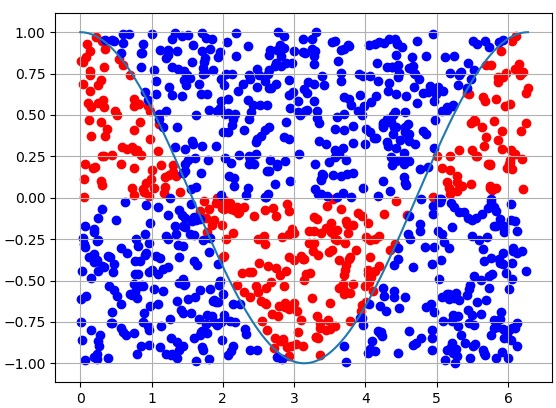
\includegraphics{Points}
        \caption{Какий-та точки}
    \end{figure}

    \section{Second section}

    Hello, here is some text without a meaning.  This text should show what 
    a printed text will look like at this place.  If you read this text, 
    you will get no information.  Really?  Is there no information?  Is there 
    a difference between this text and some nonsense like not at all!  A 
    blind text like this gives you information about the selected font, how 
    the letters are written and an impression of the look.  This text should
    contain all letters of the alphabet and it should be written in of the
    original language.There is no need for special content, but the length of
    words should match the language.

    \begin{table}[H]
            
        \caption{Какий-та буквы}
        \noindent\begin{tabular}{|c|c|c|c|c|c|c|c|}
            \hline
            cell & cell & cell & cell & cell & cell & cell & cell \\
            cell & cell & cell & cell & cell & cell & cell & cell \\
            cell & cell & cell & cell & cell & cell & cell & cell \\
            \hline
            
        \end{tabular}

    \end{table}

    \subsection{Second section first subsection}

    Hello, here is some text without a meaning.  This text should show what 
    a printed text will look like at this place.  If you read this text, 
    you will get no information.  Really?  Is there no information?  Is there 
    a difference between this text and some nonsense like not at all!  A 
    blind text like this gives you information about the selected font, how 
    the letters are written and an impression of the look.  This text should
    contain all letters of the alphabet and it should be written in of the
    original language.There is no need for special content, but the length of
    words should match the language.

\end{document}